\documentclass[nobib]{tufte-handout}

\title{Funkcijų transformacijos}

\author[Vilius Paliokas]{Vilius Paliokas}

\date{2023-02-01} % without \date command, current date is supplied

%\geometry{showframe} % display margins for debugging page layout

\usepackage[main=lithuanian]{babel}
\usepackage[utf8]{inputenc}

\usepackage{tikz}
\usepackage{tikz-cd}
\usepackage{pgfplots}

\usepackage{tasks}
\pgfplotsset{compat=1.18}
\usepackage{booktabs}
\usepackage{siunitx}

\usepackage{graphicx} % allow embedded images
\setkeys{Gin}{width=\linewidth,totalheight=\textheight,keepaspectratio}
\graphicspath{{graphics/}} % set of paths to search for images
\usepackage{amsmath}  % extended mathematics
\usepackage{booktabs} % book-quality tables
\usepackage{units}    % non-stacked fractions and better unit spacing
\usepackage{multicol} % multiple column layout facilities
\usepackage{lipsum}   % filler text
\usepackage{fancyvrb} % extended verbatim environments
\fvset{fontsize=\normalsize}% default font size for fancy-verbatim environments

% Standardize command font styles and environments
\newcommand{\doccmd}[1]{\texttt{\textbackslash#1}}% command name -- adds backslash automatically
\newcommand{\docopt}[1]{\ensuremath{\langle}\textrm{\textit{#1}}\ensuremath{\rangle}}% optional command argument
\newcommand{\docarg}[1]{\textrm{\textit{#1}}}% (required) command argument
\newcommand{\docenv}[1]{\textsf{#1}}% environment name
\newcommand{\docpkg}[1]{\texttt{#1}}% package name
\newcommand{\doccls}[1]{\texttt{#1}}% document class name
\newcommand{\docclsopt}[1]{\texttt{#1}}% document class option name
\newenvironment{docspec}{\begin{quote}\noindent}{\end{quote}}% command specification environment

\begin{document}

\maketitle% this prints the handout title, author, and date

\begin{abstract}
  \noindent
  Šioje mokomojoje medžiagoje funkcijų transformacijų teoriją ir pavyzdžius.
  Pagal bendrojo ugdymo 11 klasės matematikos bendrojo kurso programą mokiniai
  turi mokėti, kaip atliekamos $y=f(x)+a$, $y=f(x+a)$, $y=-f(x)$, $y=a\cdot
    f(x)$
  formulėmis aprašomos transformacijos. Čia taip pat pateikiamos šių
  transformacijų pasireiškimai įvairaus konteksto situacijose. Funkcijų
  transformacijoms suprasti, pirmiausia plėtojama samprata apie funkcijas ir jų
  savybes.
\end{abstract}

% \printclassoptions
\section{Funkcijos samprata}\label{se c:page-layout}

Dažnu atveju, funkcija yra asocijuojama su $f(x)$ žymėjimu, o šį mes skaitome
\textit{ef nuo iks}. Po $f(x)$ visada seka kažkoks tai
reiškinys, dažniausiai tai būna tiesinis reiškinys $ax+b$ (pvz.:
$f(x)=x+1$) ar
kvadratinis reiškinys $ax^2+bx+c$ (pvz.: $f(x)=x^2$). O vėliau, mokyklos kurse
sutiksime ir kitokio
tipo funkcijas.

Toliau prisiminsime apie aibes ir pamatysime, kaip jos susijusios su
funkcijomis.

\subsection{Apie aibes}\label{sec:about_sets}

Kadangi jau susipažinome su aibėmis, galime pasigilinti, kaip aibės
susijusios su funkcijomis. Bet pirma prisiminsime keletą aibių
teorijos\footnote{Aibių teorija yra matematikos šaka, kurioje nagrinėjamos
  aibės - objektų rinkiniai} aspektų. \textbf{Aibė} - rinkinys	objektų, kurie
vadinasi aibės elementais. Aibės elementu gali būti bet kas (obuoliai,
planetos, mašinos), o jie yra susieti viena (ar daugiau) bendra
savybę. Matematikoje nagrinėjami matematiniai objektai, mokyklos matematikos
programoje nagrinėjamos
tik skaičių aibės. Jeigu elementas $x$ priklauso aibei $X$, tai užrašoma $x \in
  X$. Jeigu elementas $x$ nepriklauso aibei $X$, tai rašome $x \notin X$.

Priklausomai nuo elementų skaičiaus aibėje, aibės gali būti baigtinės arba
begalinės. Baigtinės aibės atveju mes galime suskaičiuoti šios elementus, juos
nesunkiai visus išvardinti. Pavyzdžiui turime aibę
$$A=\{0; 1; 4; 9; 16; 25\} $$
Ši aibė turi baigtinį kiekį elementų - ją sudaro 6 elementai. Natūraliųjų
skaičių aibė $\mathbb{N}$ yra vienas iš begalinės aibės pavyzdžių, ši aibė turi
be galo daug
elementų ($1;2;3;4;5;6;7;8\ldots$).

\subsection{Aibės ir funkcijos}\label{sec:about_sets_and_functions}

O dabar bandysime atsakyti į klausimą, kaip susijusios aibės ir funkcija.
Tarkime turime dvi aibes $X$ ir $Y$ (paskui bus ir konkretūs pavyzdžiai).
Paprastumo dėlei, šios aibės bus baigtinės abi sudarytos iš keturių elementų:

$$X = \{x_{1},x_{2},x_{3},x_{4}\};$$
$$Y = \{y_{1},y_{2},y_{3},y_{4}\};$$

Šių grafinis atvaizdavimas pažymėtas žemiau,
\ref{fig:function_as_sets_elements_relation} paveiksle. Kol kas pavaizduotas
rodykles ignoruokime.

\begin{figure}[!htpb]
  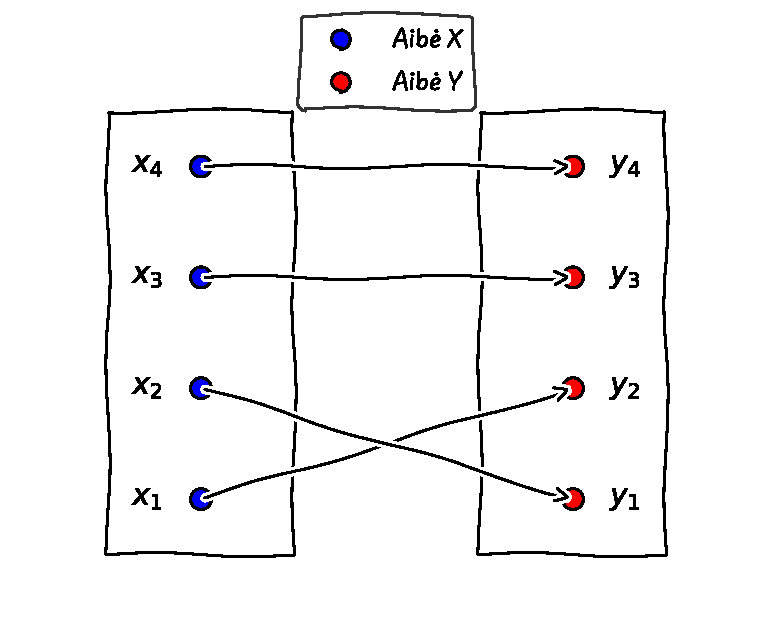
\includegraphics{./graphs/functions_as_graphs.pdf}
  \caption{Funkcija, kaip aibių elementų sąryšiai}
  \label{fig:function_as_sets_elements_relation}
  \setfloatalignment{c}
\end{figure}

O dabar svarbiausia dalis. Kiekvienam aibės $X$ elementui priskyrus elementą iš
aibės $Y$ gauname tam tikrus ryšius tarp šių dviejų aibių. Tarkime, anksčiau
paminėtiems elementams iš aibės $X$ priskirkime elementą iš aibės $Y$:
\begin{itemize}
  \item $x_1 \rightarrow y_2$;
  \item $x_2 \rightarrow y_1$;
  \item $x_3 \rightarrow y_3$;
  \item $x_4 \rightarrow y_4$;
\end{itemize}

Šiuos ryšius tarp dviejų aibių elementų galime matyti
\ref{fig:function_as_sets_elements_relation} paveiksle, jie pavaizduoti
rodyklėmis. Rodyklė $\rightarrow$ yra priskirimo veiksmas matematikoje. Jeigu
visų aibės $X$ elementų priskyrimo aibės $Y$ elementams veiksmą pavadintume
$f$, tai galėtume
pažymėti:
$$ f: X \rightarrow Y  \quad\text{arba}\quad  X \xrightarrow{f} Y$$

Iki šio momento turėjote pamatyti pažįstamų dalykų: $f$, $x$, $y$. Jei
kiekvienas aibės $X$ elementas yra susijęs su vienu ir tik vienu kitos aibės
$Y$ elementu, tai toks priskyrimas (ryšys) vadinamas
\textbf{funkcija}\footnote{Labai
  svarbi šio apibrėžimo dalis yra ta, kad vienas (ir tik vienas) elementas
  priskiriamas kitam aibės elementui, kitu atveju tai negali vadintis
  funkcija}. O tai užrašoma $y=f(x)$.

\subsection{Funkcijos sąvokos}\label{sec:function_related_defintions}

Kalbant apie funkcijas, būtina žinoti su funkcija susijusiąs sąvokas. Šios
sąvokos ateina iš funkcijos apibrėžimo:

\begin{itemize}
  \item $x$ - funkcijos nepriklausomas kintamasis arba funkcijos argumentas;
  \item $y$ - funkcijos priklausomas kintamasis arba funkcijos reikšmė;
  \item $X$ - visos galimos $x$ reikšmės arba funkcijos $f(x)$ apibrėžimo
        sritis. Ši sritis dažnai žymima $D(f)$;
  \item $Y$ - visos galimos $y$ reikšmės arba funkcijos $f(x)$ reikšmių sritis.
        Ši sritis dažnai žymima $E(f)$;
  \item $f$ - taisykė, pagal kurią $x$ reikšmėms priskiriamos $y$ reikšmės;
\end{itemize}

Šių sąvokų atikmenis galima pamatyti anksčiau pavaizduotame
\ref{fig:function_as_sets_elements_relation} paveiksle. Pavyzdžiui, paveiksle
mėlyni rutuliukai $x_1, x_2, x_3, x_4$ yra funkcijų argumentai, o jų visuma
(apibrėžta sritis) yra apibrėžimo sritis. Reikšmių sritis yra apibrėžta sritis
su raudonai $y_1, y_2, y_3, y_4$ taškais. Visų rodyklių visuma yra taisyklė
$f$, pagal kurią vieni aibės (apibrėžimo srities) elementai priskiriami kitiems
aibės (reikšmių srities) elementams.

\subsection{Funkcijos pavyzdys}\label{sec:function_example}

Turime dvi aibes:
$$X =\{0; 1; 2; 3; 4; 5\}$$
$$Y =\{0; 1; 4; 9; 16; 25\}$$

Dabar priskirkime aibės $X$ vienam ir tik vienam kitos aibės $Y$ elementą:
\begin{itemize}
  \item $0 \rightarrow 0$;
  \item $1 \rightarrow 1$;
  \item $2 \rightarrow 4$;
  \item $3 \rightarrow 9$;
  \item $4 \rightarrow 16$;
  \item $5 \rightarrow 25$;
\end{itemize}

Šį priskyrimą pavadinkime $f$. Dabar, šių skaičių ryšį galima parašyti $y=f(x)$
arba $f(x)=y$  forma:
\begin{itemize}
  \item $f(0) = 0$;
  \item $f(1) = 1$;
  \item $f(2) = 4$;
  \item $f(3) = 9$;
  \item $f(4)= 16$;
  \item $f(5) = 25$;
\end{itemize}

Šiuos ryšius galima pavaizduoti ir grafiškai:

\begin{figure}[!htpb]
  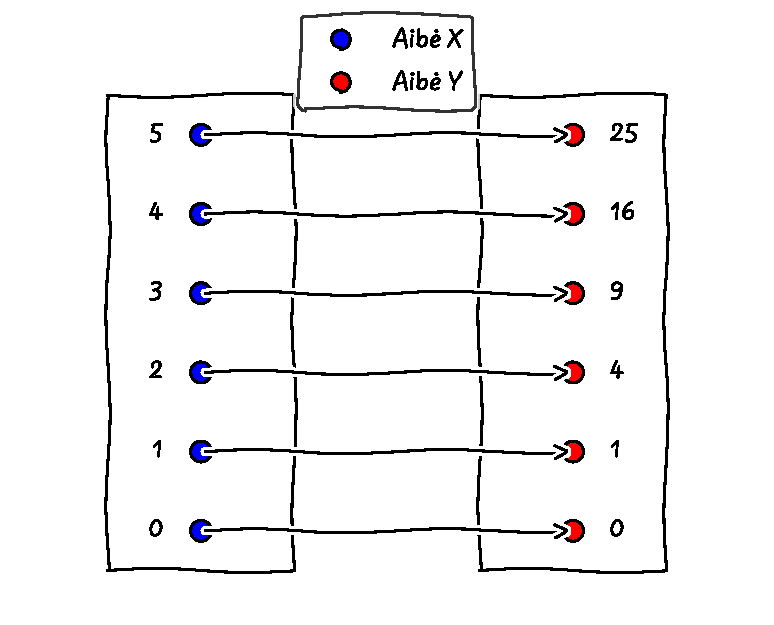
\includegraphics{./graphs/functions_as_graphs_example1.pdf}
  \caption{Aibės $X =\{0; 1; 2; 3; 4; 5\}$ elementų priskyrimas aibės $Y =\{0;
      1; 4; 9; 16; 25\}$ elementams}
  \label{fig:function_as_set_example}
  \setfloatalignment{c}
\end{figure}

Šią funkcinę priklausomybę galima ir apibūdinti:
\begin{itemize}
  \item Funkcijos apibrėžimo sritis yra $\{0; 1; 2; 3; 4; 5\}$;
  \item Funkcijos reikšmių sritis yra $\{0; 1; 4; 9; 16; 25\}$;
  \item Mažiausia reikšmė ($y$) yra 0, kai argumentas ($x$) yra lygus 0;
  \item Didžiausia reikšmė ($y$) yra 25, kai argumentas ($x$) yra lygus 5;
\end{itemize}

\subsection{Funkcijos reiškinys}\label{sec:function_example}

Funkciją galima aprašyti reiškiniu. Ta daroma, nes neįmanoma išrašyti visų
begalinių ryšių tarp dviejų begalinių aibių. Šiuos reiškinius jau analizavote
ir ankstesnėse klasėse. Anksčiau pateiktame pavyzdyje, galima įžvelgti tam
tikrą dėsningumą. Funkcijos reikšmės buvo gautos argumentus pakėlus kvadratu.
Tokią bendrą taisyklę visiems skaičiams ($x\in \mathbb{R}$) galima užrašyti
taip:
$$f(x)=x^2$$

\begin{marginfigure}%

  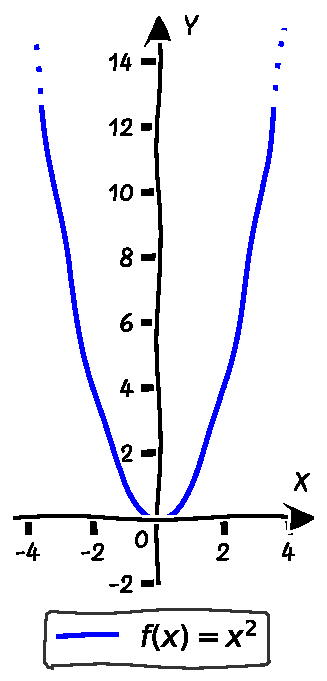
\includegraphics[width=\linewidth]{./graphs/quadratic_function_plot_example.pdf}
  \caption{$f(x)=x^2$ grafikas $OXY$ koordinačių plokštumoje}
  \label{fig:example_quadratic_plot}
\end{marginfigure}

Tai reiškia, kad kiekviena funkcijos reikšmė gaunama argumentą, iš apibrėžimo
srities, pakėlus kvadratu. Tokiu būdu gaunama begalė argumentų $x$ ir reikšmių
$y$ skaičių porų
$(x; y)$. Šiuos taškus atvaizdavus koordinačių plokštumoje $OXY$ gaunamas
funkcijos grafikas (\hyperref[fig:example_quadratic_plot]{paveikslas
  \ref*{fig:example_quadratic_plot}}).

\section{Grafikų transformacija}\label{sec:graph_transformation}

Tarkime turime žinome, kaip atrodo funkcijos grafikas, jį modifikuojame taip,
kad sukurtume panašus, bet kitoks to grafikos variantas. Toks procesas
vadinamas funkcijos grafiko transformacija. Matematikos bendrajame kurse reikia
žinoti 4 tipų transformacijas. Šių transformacijų pavyzdžiai matomi žemiau:

\begin{figure*}[h]
  \begin{minipage}{0.19\textwidth}
    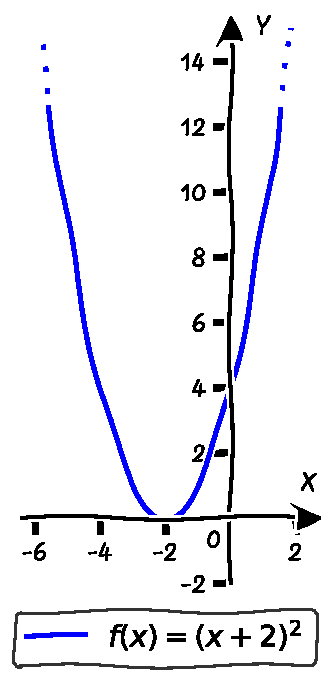
\includegraphics[width=\linewidth]{./graphs/quadratic_func_lsh_2.pdf}
    \label{fig:first}
  \end{minipage}\hfill
  \begin{minipage}{0.19\textwidth}
    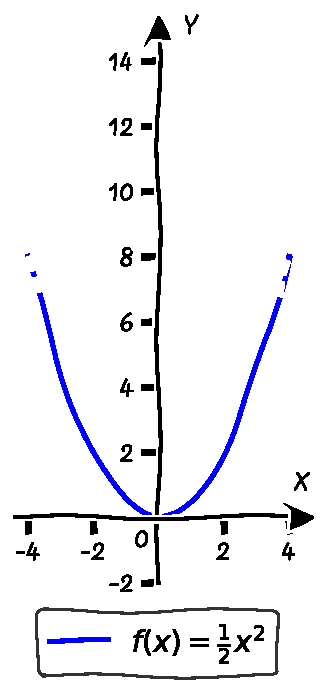
\includegraphics[width=\linewidth]{./graphs/quadratic_func_shrink_2.pdf}
    \label{fig:second}
  \end{minipage}\hfill
  \begin{minipage}{0.19\textwidth}
    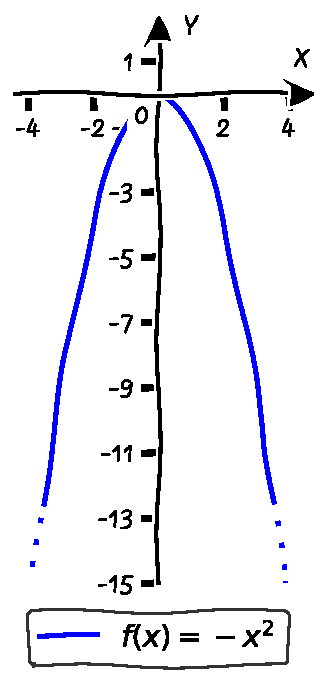
\includegraphics[width=\linewidth]{./graphs/quadratic_func_flipped.pdf}
    \label{fig:third}
  \end{minipage}\hfill
  \begin{minipage}{0.19\textwidth}
    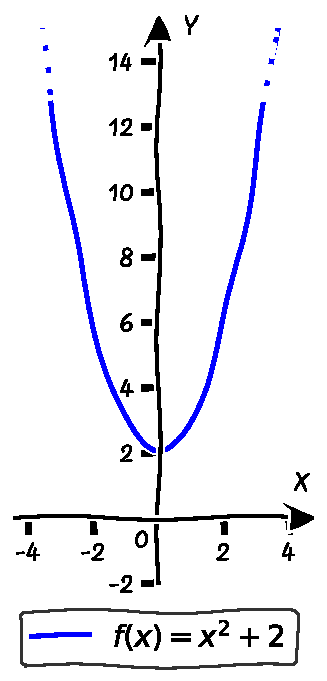
\includegraphics[width=\linewidth]{./graphs/quadratic_func_ush_2.pdf}
    \label{fig:fourth}
  \end{minipage}
  \caption{$f(x)=x^2$ grafiko transformacijos: $y=f(x-2)$, $y=\frac{1}{2}f(x)$,
    $y=2f(x)$, $y=f(x)+2$ }
\end{figure*}

Šie visi grafikai atrodo panašiai, bet skiriasi nuo pradinės funkcijos
$f(x)=x^2$ grafiko, nes atlitkos tam tikros transformacijos:

\begin{itemize}
  \item Postūmis OX ašimi $y=f(x+a)$, čia $a \in \mathbb{R}$;
  \item Postūmis OY ašimi $y=f(x)+b$, čia $b \in \mathbb{R}$;
  \item Ištempimas, sutraukimas $y=c \cdot\ f(x)$, čia $c \in \mathbb{R}$;
  \item Apvertimas OX ašies atžvilgiu $y=-f(x)$;
\end{itemize}

Toliau giliau analizuosime šių transformacijų poveikį grafikams, jų taškams.
Įsivaizduokime turime funkcijos $f(x)$ tašką $(a, b)$, tai tokiu atveju $f(a) =
  b$. \hyperref[tbl:after_transformations]{\ref*{tbl:after_transformations}
  lentelėje
} pavaizduota, kaip keičiasi funkcijos taškai $(a, b)$ ir grafikas,
modifikuojant
funkcijos $f(x)$ reikšmę.

\begin{table*}[!htpb]
  \centering
  \begin{tabular}{
      S |
      S[separate-uncertainty = true] |
      S[table-format = 5]
    }
    \toprule
    Transformacija                    & {Kaip pasikeičia $f(x)$ grafiko
        taškai}
                                      & {Grafiko vizualinis pokytis}        \\
    \midrule
    {$f(x)+d$, $d>0$}                 & {$(a,b)\mapsto(a, b+d)$}
                                      & {Kyla viršun per $d$}               \\
    {$f(x)-d$, $d>0$}                 & {$(a,b)\mapsto(a, b-d)$}
                                      & {Leidžiasi žemyn per $d$}           \\
    {$c \cdot f(x)$, $c>0$}           & {$(a,b)\mapsto(a, c \cdot b)$}
                                      & {Išsitempia vertikaliai per $c$}    \\
    {$\frac{1}{c} \cdot f(x)$, $c>0$} & {$(a,b)\mapsto(a, \frac{1}{c} \cdot
          b)$}
                                      & {Susitraukia vertikaliai per $c$}   \\
    {$-f(x)$}                         & {$(a,b)\mapsto(a, -b)$}
                                      & {Apsiverčia $OX$ ašies atžvilgiu}   \\
    \bottomrule
  \end{tabular}
  \vspace{16pt} % Adjust the space as needed
  \caption{Funkcijų transformacijos, modifikuojant jos reikšmę}.
  \label{tbl:after_transformations}
\end{table*}

\subsection{Pavyzdys}\label{sec:function_transformation_example}

Pavaizduosime konkrečius pavyzdžius
aprašytoms transformacijoms
\hyperref[tbl:after_transformations]{\ref*{tbl:after_transformations}
  lentelėje}. Tam naudosime jau anksčiau naudotą $f(x)=x^2$ funkciją.
Pažiūrėsime, koks pokytis, kai nubrėžus $f(x)+2$,  $f(x)-2$,
$2f(x)$,$\frac{1}{2}f(x)$,$-f(x)$. Šiuos brėžinius rasite
\hyperref[sec:function_transformation_example]{\pageref*{fig:function_transformation_example}
  puslapyje}.

Matome, kad padvigubinus funkcijos $f(x)$ reikšmę ($2 \cdot f(x)$),
ji išsitempia, o taškų $y$ koordinatės reikšmės padvigubėja, pavyzdžiui taškas
$(2; 4)$ tapo $(2;4 \cdot 2)=(2;8)$

Pridėjus prie $f(x)$ reikšmių 2, gauname paslinkta grafiką per du vienetus
aukštyn. Visų taškų $y$ reikšmė padidėja per du vienetus. Pavyzdžiui taškas
$(2; 4)$ tapo $(2;4 + 2)=(2;6)$

Grafiką galime sutraukti, jis tampa plokštesnis. Tai padarėme funkciją $f(x)$
padauginus iš $\frac{1}{2}$. Visos taškų $y$ reikšmės sumažėjo perpus. Taškas
$(2; 4)$ tapo $(2;4 \cdot \frac{1}{2})=(2;2)$

Kaip paslinkome grafiką aukštyn, taip galima ir paslinkti žemyn. Tą padarome
atimdami (arba pridėdami neigiamą reikšmę) iš funkcijos $f(x)$. Pavyzdyje
funkcijos $f(x)-2$ grafikas skiriasi tuo, kad jis pasislinkęs žemyn per du
vienetus - visi taškų oordinatės\footnote{Plokštumos taškai $(x;y)$
matematikoje dar vadinami abcise ir ordinate: $
  (\overbrace{x}^{\text{abscisė}};
  \overbrace{y}^{\text{ordinatė}})$} reikšmė sumažinta per du
vienetus.

Paprasčiausia transformacija - apvertimas $OX$ ašies atžvilgiu.
Šios principus palieku išsiaiškinti savarankiškai.

\begin{figure*}[p]
  \begin{fullwidth}
    \centering
    % First row
    \hspace*{-205pt} % Adjust this value as needed
    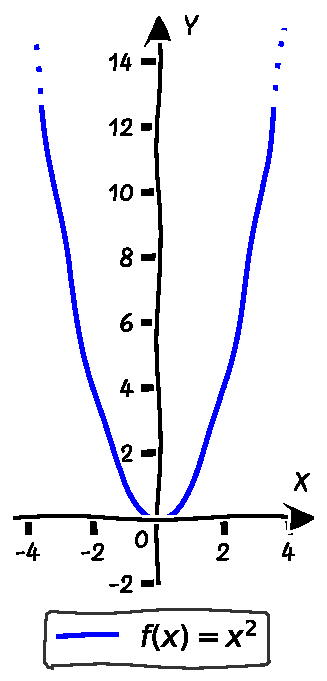
\includegraphics[width=0.23\linewidth]{./graphs/quadratic_func_primary.pdf}

    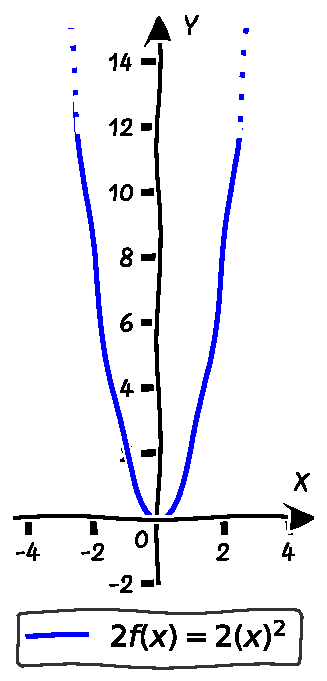
\includegraphics[width=0.23\linewidth]{./graphs/quadratic_func_transform_2.pdf}\hspace{5pt}

    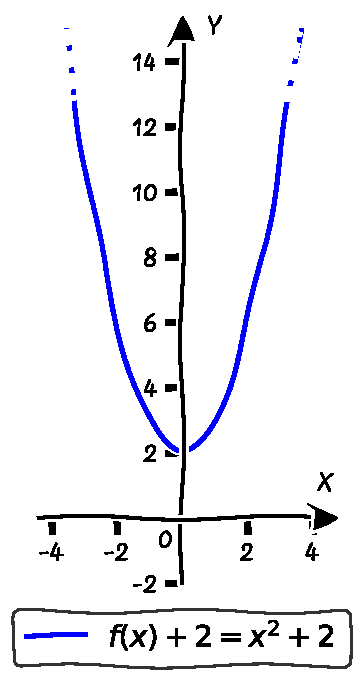
\includegraphics[width=0.25\linewidth]{./graphs/quadratic_func_transform_3.pdf}
    \\\vspace{\baselineskip}

    % Second row
    \hspace*{-205pt} % Keep this value consistent with the first row

    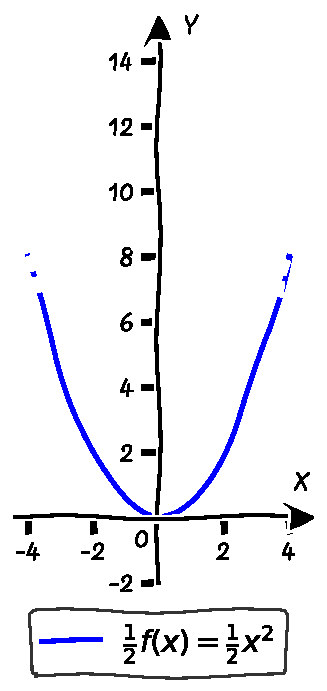
\includegraphics[width=0.23\linewidth]{./graphs/quadratic_func_transform_4.pdf}\hspace{5pt}

    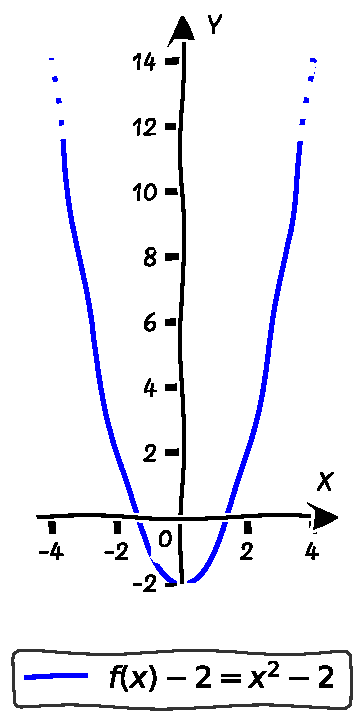
\includegraphics[width=0.24\linewidth]{./graphs/quadratic_func_transform_5.pdf}\hspace{5pt}

    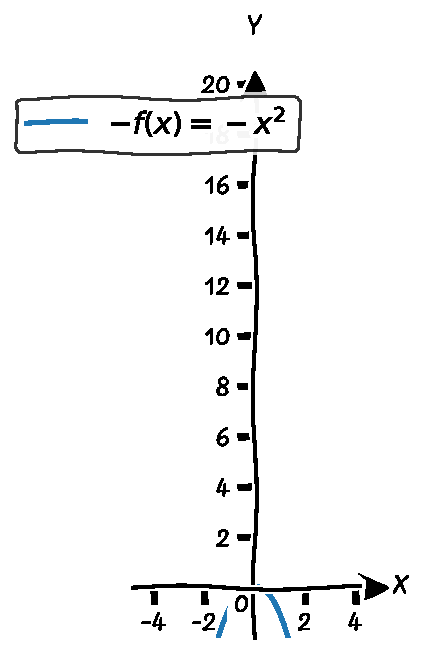
\includegraphics[width=0.23\linewidth]{./graphs/quadratic_func_transform_6.pdf}
  \end{fullwidth}
  \label{fig:function_transformation_example}
\end{figure*}

\subsection{Postūmiai OX ašimi}\label{sec:translation_OX_axis}

Liko išsiaiškinti dar du postūmių tipus: grafiko slinkimą kairėn ir dešinėn OX
ašimi.

\begin{table}[!htpb]
  \centering
  \begin{tabular}{
    l | % Left-aligned
    >{\raggedleft\arraybackslash}p{3cm} | % Right-aligned with fixed width
    r	% Right-aligned with fixed width
    }
    \toprule
    {Transformacija}  & {Kaip pasikeičia $f(x)$ grafiko taškai}
                      & {Grafiko vizualinis pokytis}            \\
    \midrule
    {$f(x+d)$, $d>0$} & {$(a,b)\mapsto(a-d, b)$}
                      & {Pasislenka į kairę per $d$}            \\
    {$f(x-d)$, $d>0$} & {$(a,b)\mapsto(a+d, b)$}
                      & {Pasislenka į dešinę per $d$}           \\
    \bottomrule
  \end{tabular}
  \vspace{16pt} % Adjust the space as needed
  \caption{Funkcijų transformacijos, modifikuojant jos argumentą $x$}
  \label{tbl:after_transformations}
\end{table}

Vėl paanalizuosime funkciją $f(x)$ ir poslinkis, kai pridedame skaičių prie
argumento
arba atimame skaičių prie argumento. Dvi skirtingas transformacijas -
poslinkius $OX$ ašies kryptimi rasite dešinėje pusėje,
\hyperref[fig:quadratic_func_transform_lshifted_2]{paveiksle
  \ref*{fig:quadratic_func_transform_lshifted_2}} ir
\hyperref[fig:quadratic_func_transform_rshifted_2]{paveiksle
  \ref*{fig:quadratic_func_transform_rshifted_2}}. Pažvelgus į grafikus, turėtų
atrodyti neintuityviai, prieštaringai, kad padidinus argumentą $x$ dviem,
grafikas pasislinko į kairę pusę per dvi vietas. Šiuo atveju kiekvienas taškas
$(a;b)$ tapo $(a-2;b)$. Tokia pat situacija su kita transformacija. Atėmus 2
prie argumento $x$, grafikas pasislinko į dešinę pusę.

\begin{marginfigure}%

  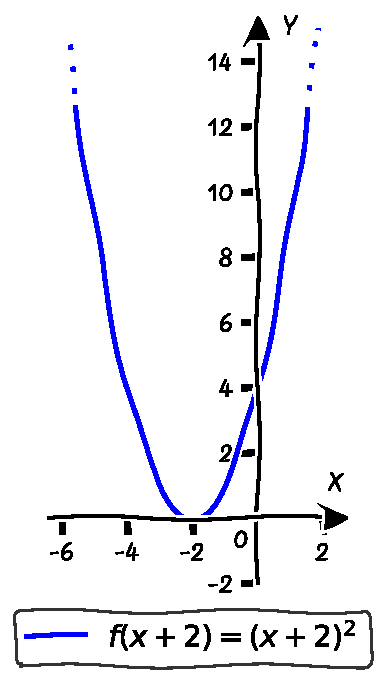
\includegraphics[width=\linewidth]{./graphs/quadratic_func_transform_lshifted_2.pdf}
  \caption{$f(x)=x^2$ funkcijos transformacija $f(x+2)=(x+2)^2$}
  \label{fig:quadratic_func_transform_lshifted_2}
\end{marginfigure}

\begin{marginfigure}%

  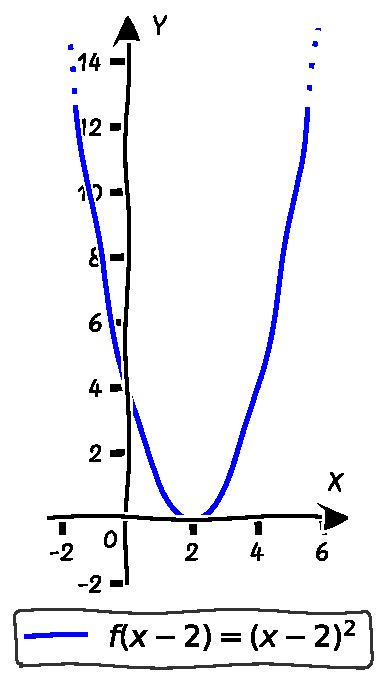
\includegraphics[width=\linewidth]{./graphs/quadratic_func_transform_rshifted_2.pdf}
  \caption{$f(x)=x^2$ funkcijos transformacija $f(x-2)=(x-2)^2$}
  \label{fig:quadratic_func_transform_rshifted_2}
\end{marginfigure}

Tad šitą principą reiktų įsiminti:
\begin{center}
  \textbf{Prie argumento pridedant, graifkas juda į kairę,\\ atimant iš
    argumento, grafikas juda į dešinę}.
\end{center}

Grafikų transformacijas galima jungti tarpusavyje: apversti, paslinkti į dešinę
per $n$, nuleisti žemyn per $m$, ištempti. Pavyzdžiui turime tiesinę funkciją
$$f(x)=x$$
tai šią galima paslinkti į kairę per 2, pakelti per 5, apversti ir
ištempti 3 vienetais. Tokia transformacija užsirašys šitaip:

$$-3f(x+3)+5=-3(x-3)+5$$

Tokius atvejus pasižiūrėsime toliau, uždaviniuose.
\section{Uždaviniai}\label{sec:exercises}

\begin{enumerate}
  \item Funkcija $f(x)$ paslinkta per 3 vienetus į kairę ir 4 vienetus aukštyn.
        Paraškite naujosios funkcijos reiškinį.
  \item Turime pradinę funkciją $f(x)=-3x-6$, šiai funkcijai buvo atlikta
        kombinacija transformacijų ir gauta $g(x)=x+2$. Nurodykite kokios
        transformacijos buvo atlitkos funkcijai $f(x)$.
  \item (\textit{Iš išplėstinio kurso knygos, 361 užduotis}) Parašykite
        funkcijos $y=g(x)$ reiškinį $g(x)$:

        \begin{tasks}[item-format={\normalfont}, after-item-skip=2mm](2)
          \task $g(x)=f(x)-2$,\\ $f(x)=7x^2$;
          \task $g(x)=f(x-3)$,\\  $f(x)=\frac{9}{x}$;
          \task $g(x)=f(x-2)+1$,\\  $f(x)=-\frac{2}{x}$;
          \task $g(x)=f(x+2)-3$,\\ $f(x)=\frac{1}{3}x^2$;
        \end{tasks}

  \item (\textit{Iš išplėstinio kurso knygos, 356 užduotis, modifikuota})
        Pavaizduotas
        (\hyperref[fig:4_exercise_graph]{paveikslas
          \ref*{fig:4_exercise_graph}})
        funkcijos $y=f(x)$ grafikas. Nubraižykite funkcijos $y=g(x)$ grafiką,
        kai:

        \begin{marginfigure}%

          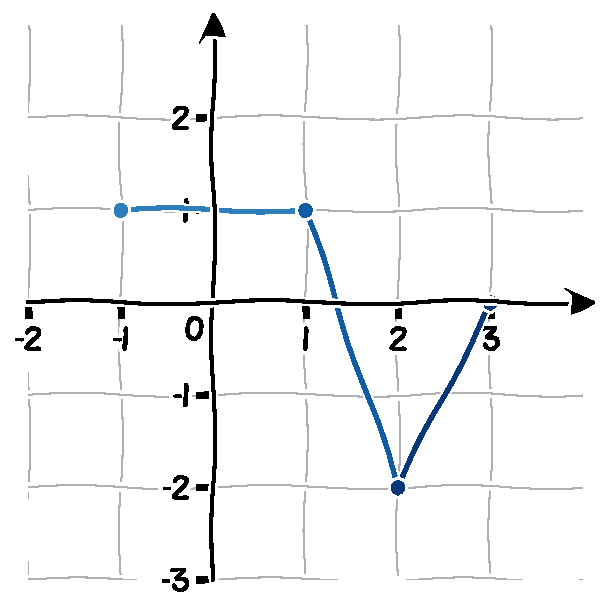
\includegraphics[width=\linewidth]{./graphs/exercise_4_plot.pdf}
          \caption{4 užduoties funkcijos $y=f(x)$ grafikas}
          \label{fig:4_exercise_graph}
        \end{marginfigure}

        \begin{tasks}[item-format={\normalfont}, after-item-skip=2mm](2)
          \task $g(x)=f(x-1)-3$;
          \task $g(x)=f(x+1)-2$;
          \task $g(x)=-3f(x-2)+1$;
          \task $g(x)=\frac{1}{2}f(x+2)-3$;
        \end{tasks}

  \item Pagal 4 užduotį, nurodykite funkcijos apibrėžimo
        sritį, reikšmių sritį, mažiausią ir didžiausią reikšmes.
        \begin{tasks}[item-format={\normalfont}, after-item-skip=2mm](2)
          \task $f(x)$;
          \task $g(x)=f(x-1)-3$;
          \task $g(x)=f(x+1)-2$;
          \task $g(x)=-3f(x-2)+1$;
          \task $g(x)=\frac{1}{2}f(x+2)-3$;
        \end{tasks}

  \item Parašykite funkciją, atitinkančią $g(x)$ grafiką, kuris transformavosi
        iš
        $f(x)$ grafiko taikant funkcijų transformavimo taisykles
        (\hyperref[fig:6_exercise_plots]{paveikslas
          \ref*{fig:6_exercise_plots}}).

        \begin{marginfigure}%

          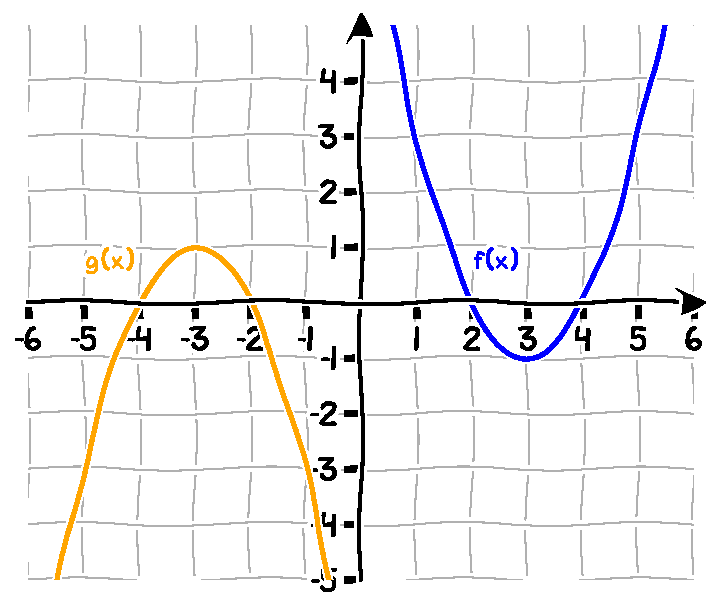
\includegraphics[width=\linewidth]{./graphs/exercise_6_two_functions.pdf}
          \caption{6 užduoties funkcijų $y=f(x)$ ir $y=g(x)$ grafikai}
          \label{fig:6_exercise_plots}
        \end{marginfigure}

  \item Pagal 6 užduotį, nurodykite funkcijų $y=f(x)$ ir $y=g(x)$ apibrėžimo
        sritis, reikšmių sritis, mažiausias ir didžiausias reikšmes.

  \item (\textit{Iš matematikos bendrojo kurso pirmojo tarpinio patikrinimo
          užduoties pavyzdžio}). \hyperref[fig:8_exercise_sine_wave]{Paveiksle
          \ref*{fig:8_exercise_sine_wave}} pavaizduotas funkcijos
        $f(x)=\sin{x}$ grafiko eskizas. Nustatykite funkcijos $g(x)=5-\sin{x}$
        didžiausią ir mažiausią reikšmę.
        \begin{figure}[!htpb]

          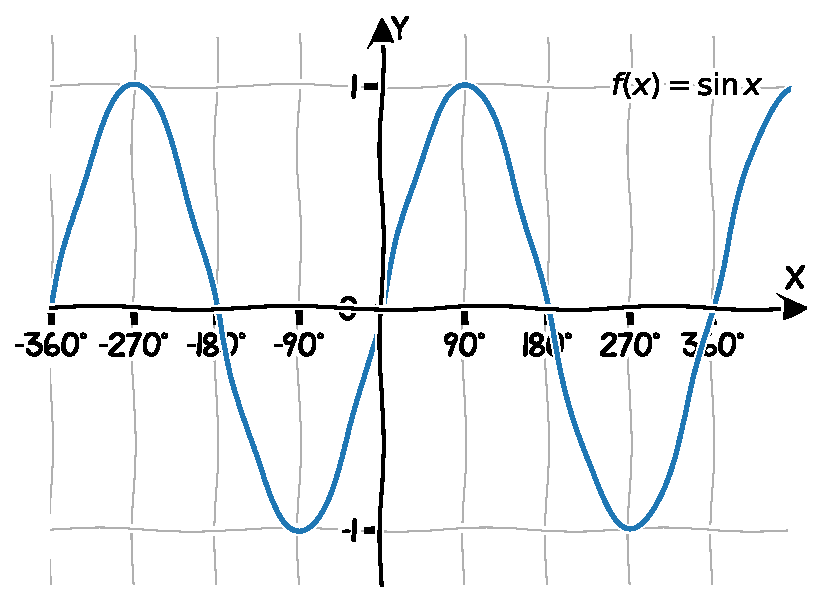
\includegraphics[width=.825\linewidth]{./graphs/exercise_8_sin_wave.pdf}
          \caption{Funkcijos $f(x)=\sin{x}$ grafiko eskizas}
          \label{fig:8_exercise_sine_wave}
          \setfloatalignment{c}
        \end{figure}
\end{enumerate}

\clearpage



\end{document}
